\documentclass{beamer}
\usetheme{Boadilla}

\newcommand{\mb}{\overline{\mathcal M}}
\newcommand{\mgn}{\mathcal M_{g,n}}
\newcommand{\mgnb}{\mb_{g,n}}
\newcommand{\mgb}[1]{\mb_{g,#1}}
\usepackage{amsmath}                % give more fonts and symbols
\usepackage{amsfonts}               % want AMS fonts
\usepackage{amssymb}
\usepackage{amsthm}
\usepackage{mathrsfs}
\usepackage{tikz-cd}
%\usepackage[shortlabels]{enumitem}
\usepackage{tocbasic}
\usepackage{hyperref}
\usepackage{biblatex}
\usepackage{listings}
\addbibresource{sources.bib}

% Some letter symbols
\newcommand{\N}{\ensuremath{\mathbb{N}}}
\newcommand{\Z}{\ensuremath{\mathbb{Z}}}
\newcommand{\R}{\ensuremath{\mathbb{R}}}
\newtheorem*{Proposition}{Proposition}
%\newtheorem*{Corollary}{Corollary}
\newcommand{\Q}{\mathbb{Q}}
\newcommand{\C}{\mathbb{C}}
\newcommand{\Aut}{\text{Aut}}
\newcommand{\codim}{\text{codim}}
\newcommand{\exer}[1]{{\bf Exercise #1} \\}
\newcommand{\Hom}{\text{Hom}}
\newcommand{\Hb}{\overline{\mathcal H}}
\renewcommand{\a}{\mathfrak a}
\renewcommand{\b}{\mathfrak b}
\renewcommand{\P}{\mathbb P}
\theoremstyle{definition}
\newtheorem{thm}{Theorem}[section]
\newtheorem{cor}[thm]{Corollary}
\newtheorem{dfn}[thm]{Definition}
\newtheorem{claim}[thm]{Claim}
\newtheorem{prop}[thm]{Proposition}
\newtheorem{lem}[thm]{Lemma}
\newtheorem{eg}[thm]{Example}

\usetikzlibrary{matrix,positioning,quotes}

%==============================================================================
% YOUR DOCUMENT (start here)
%==============================================================================

\definecolor{myblue}{RGB}{100,180,255}
\definecolor{mygreen}{RGB}{80,160,80}
\definecolor{myred}{RGB}{200,120,100}

\usepackage{amsmath, amssymb}

%\usefonttheme{professionalfonts}
%\setbeamertemplate{navigation symbols}{}

% --- page number ---
%\setbeamertemplate{footline}{%
%	\raisebox{10pt}{\makebox[\paperwidth]{\hfill\makebox[7em]{\normalsize\texttt{\insertframenumber/\inserttotalframenumber}}}}%
%}


\title{Reverse Hurwitz counts of genus $1$ curves}
\author{Michael Mueller}
\date{\today}

\setbeamertemplate{itemize items}[default]
\setbeamertemplate{enumerate items}[default]

\begin{document}

    \begin{frame}[plain]
        \maketitle
    \end{frame}

        \begin{frame}{Acknowledgements}
    \end{frame}

    \begin{frame}{Outline}
      \begin{itemize}
      \item Background
      \item Thesis problem
      \item Methods
      \item All twos case
      \item $S_{\a,\b}$
      \item Future directions
        \item References
        \end{itemize}
      \end{frame}

    \begin{frame}{Enumerative geometry}

      \begin{columns}[c]
        \begin{column}{0.6\hsize}
      
          \begin{itemize}
          \item The study of counting problems in geometry
          \item Examples: \begin{itemize}
          \item How many lines contain two given points?
          \end{itemize}
          \end{itemize}
        \end{column}
        \begin{column}{0.4\hsize}

          \centering
          \vspace*{1.2in}
          
\begin{tikzpicture}
            \filldraw[color=black!60, fill=black!60](-2,0) circle (.1);
            \filldraw[color=black!60, fill=black!60](0,.3) circle (.1);
          \end{tikzpicture}
          
        \end{column}
      \end{columns}
    \end{frame}

    \begin{frame}{Enumerative geometry}

      \begin{columns}[c]
        \begin{column}{0.6\hsize}
      
          \begin{itemize}
          \item The study of counting problems in geometry
          \item Examples: \begin{itemize}
          \item How many lines contain two given points? {\color{red} 1}
          \end{itemize}
          \end{itemize}
        \end{column}
        \begin{column}{0.4\hsize}

          \centering
          \vspace*{1.2in}
          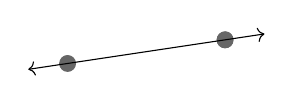
\begin{tikzpicture}
            \filldraw[color=black!60, fill=black!60](-2,0) circle (.1);
            \filldraw[color=black!60, fill=black!60](0,.3) circle (.1);
            \filldraw[color=black!60, fill=black!60](0,.3) circle (.1);
            % y = .15(x+2)
            \draw[<->] (-2.5,-.075) -- (0.5,.375);
          \end{tikzpicture}
          
        \end{column}
      \end{columns}
    \end{frame}

    \begin{frame}{Enumerative geometry}

      \begin{columns}[c]
        \begin{column}{0.6\hsize}
      
          \begin{itemize}
          \item The study of counting problems in geometry
          \item Examples: \begin{itemize}
          \item How many lines contain two given points? {\color{red} $1$}
          \item How many circles contain three given points?
          \end{itemize}
          \end{itemize}
        \end{column}
        \begin{column}{0.4\hsize}

          \centering
          \vspace*{1.2in}
          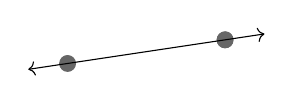
\begin{tikzpicture}
            \filldraw[color=black!60, fill=black!60](-2,0) circle (.1);
            \filldraw[color=black!60, fill=black!60](0,.3) circle (.1);
            \filldraw[color=black!60, fill=black!60](0,.3) circle (.1);
            % y = .15(x+2)
            \draw[<->] (-2.5,-.075) -- (0.5,.375);
          \end{tikzpicture}

          \vspace*{.5in}
          
\begin{tikzpicture}
            \filldraw[color=black!60, fill=black!60](-.9,-.4359) circle (.1);
            \filldraw[color=black!60, fill=black!60](-.6,.8) circle (.1);
            \filldraw[color=black!60, fill=black!60](1,0) circle (.1);
          \end{tikzpicture}
          
        \end{column}
      \end{columns}
    \end{frame}

        \begin{frame}{Enumerative geometry}

      \begin{columns}[c]
        \begin{column}{0.6\hsize}
      
          \begin{itemize}
          \item The study of counting problems in geometry
          \item Examples: \begin{itemize}
          \item How many lines contain two given points? {\color{red} $1$}
          \item How many circles contain three given points? {\color{red} $1$}
          \end{itemize}
          \end{itemize}
        \end{column}
        \begin{column}{0.4\hsize}

          \centering
          \vspace*{1.3in}
          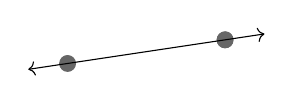
\begin{tikzpicture}
            \filldraw[color=black!60, fill=black!60](-2,0) circle (.1);
            \filldraw[color=black!60, fill=black!60](0,.3) circle (.1);
            \filldraw[color=black!60, fill=black!60](0,.3) circle (.1);
            % y = .15(x+2)
            \draw[<->] (-2.5,-.075) -- (0.5,.375);
          \end{tikzpicture}

          \vspace*{.5in}
          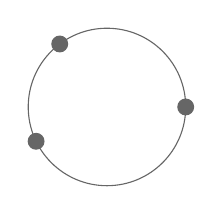
\begin{tikzpicture}
            % x^2 + y^2 = 1
            \filldraw[color=black!60, fill=white!5](0,0) circle (1);
            \filldraw[color=black!60, fill=black!60](-.9,-.4359) circle (.1);
            \filldraw[color=black!60, fill=black!60](-.6,.8) circle (.1);
            \filldraw[color=black!60, fill=black!60](1,0) circle (.1);
          \end{tikzpicture}
          
        \end{column}
      \end{columns}
        \end{frame}

        \begin{frame}{History}

      \begin{columns}[c]
        \begin{column}{0.5\hsize}
      
          \begin{itemize}
          \item {\texttildelow}200 BC: Apollonius of Perga studies circles tangent to three
            given circles
          \item {\texttildelow}1079: Omar Khayyam solves cubic equations by intersecting
            plane conics
          \item Modern enumerative geometry connects to physics (string theory),
            computer science (computer vision/cryptography), etc
            \item Circles of Apollonius:
          \end{itemize}
        \end{column}
        \begin{column}{1.1\hsize}

            \includegraphics[scale=0.23]{circle1.png}

        \end{column}
      \end{columns}
        \end{frame}

                \begin{frame}{History}

      \begin{columns}[c]
        \begin{column}{0.5\hsize}
      
          \begin{itemize}
          \item {\texttildelow}200 BC: Apollonius of Perga studies circles tangent to three
            given circles
          \item {\texttildelow}1079: Omar Khayyam solves cubic equations by intersecting
            plane conics
          \item Modern enumerative geometry connects to physics (string theory),
            computer science (computer vision/cryptography), etc
            \item Circles of Apollonius:
          \end{itemize}
        \end{column}
        \begin{column}{1.1\hsize}

            \includegraphics[scale=0.23]{circle2.png}

        \end{column}
      \end{columns}
                \end{frame}

                        \begin{frame}{History}

      \begin{columns}[c]
        \begin{column}{0.5\hsize}
      
          \begin{itemize}
          \item {\texttildelow}200 BC: Apollonius of Perga studies circles tangent to three
            given circles
          \item {\texttildelow}1079: Omar Khayyam solves cubic equations by intersecting
            plane conics
          \item Modern enumerative geometry connects to physics (string theory),
            computer science (computer vision/cryptography), etc
            \item Circles of Apollonius:
          \end{itemize}
        \end{column}
        \begin{column}{1.1\hsize}

            \includegraphics[scale=0.23]{circle3.png}

        \end{column}
      \end{columns}
                        \end{frame}

                                \begin{frame}{History}

      \begin{columns}[c]
        \begin{column}{0.5\hsize}
      
          \begin{itemize}
          \item {\texttildelow}200 BC: Apollonius of Perga studies circles tangent to three
            given circles
          \item {\texttildelow}1079: Omar Khayyam solves cubic equations by intersecting
            plane conics
          \item Modern enumerative geometry connects to physics (string theory),
            computer science (computer vision/cryptography), etc
            \item Circles of Apollonius:
          \end{itemize}
        \end{column}
        \begin{column}{1.1\hsize}

            \includegraphics[scale=0.23]{circle4.png}

        \end{column}
      \end{columns}
                                \end{frame}

                                        \begin{frame}{History}

      \begin{columns}[c]
        \begin{column}{0.5\hsize}
      
          \begin{itemize}
          \item {\texttildelow}200 BC: Apollonius of Perga studies circles tangent to three
            given circles
          \item {\texttildelow}1079: Omar Khayyam solves cubic equations by intersecting
            plane conics
          \item Modern enumerative geometry connects to physics (string theory),
            computer science (computer vision/cryptography), etc
            \item Circles of Apollonius:
          \end{itemize}
        \end{column}
        \begin{column}{1.1\hsize}

            \includegraphics[scale=0.23]{circle5.png}

        \end{column}
      \end{columns}
                                        \end{frame}

                                                \begin{frame}{History}

      \begin{columns}[c]
        \begin{column}{0.5\hsize}
      
          \begin{itemize}
          \item {\texttildelow}200 BC: Apollonius of Perga studies circles tangent to three
            given circles
          \item {\texttildelow}1079: Omar Khayyam solves cubic equations by intersecting
            plane conics
          \item Modern enumerative geometry connects to physics (string theory),
            computer science (computer vision/cryptography), etc
            \item Circles of Apollonius: $\mathbf{8}$
          \end{itemize}
        \end{column}
        \begin{column}{1.0\hsize}

            \includegraphics[scale=0.23]{circle6.png}

        \end{column}
      \end{columns}
                                                \end{frame}

                                                \begin{frame}{Broadening horizons}

      \begin{columns}[c]
        \begin{column}{0.6\hsize}
      
          \begin{itemize}
          \item Sometimes, counting problems seem to have complicated answers\dots
            \begin{itemize}
            \item Intersection points of $y = x^2$ and $y=a$ ($2$ if $a>0$,
              $1$ if $a=0$, $0$ if $a<0$)
              \item Two lines usually intersect at a point, unless they are parallel
              \end{itemize}
          \end{itemize}
        \end{column}
        \begin{column}{0.4\hsize}

          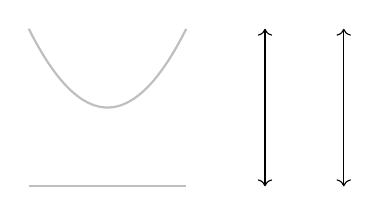
\begin{tikzpicture}
            \draw[domain=-1:1,samples=50,color=gray!50,thick] plot (\x, \x*\x);
            \draw[domain=-1:1,samples=50,color=gray!50,thick] plot (\x, -1);
            \draw[<->] (2,-1) to (2,1);
            \draw[<->] (3,-1) to (3,1);
          \end{tikzpicture}

        \end{column}
      \end{columns}
                                                \end{frame}

                                                \begin{frame}{Broadening horizons}

      \begin{columns}[c]
        \begin{column}{0.6\hsize}
      
          \begin{itemize}
          \item Sometimes, counting problems seem to have complicated answers\dots
            \begin{itemize}
            \item Intersection points of $y = x^2$ and $y=a$ ($2$ if $a>0$,
              $1$ if $a=0$, $0$ if $a<0$)
              \item Two lines usually intersect at a point, unless they are parallel
            \end{itemize}
          \item In a broader setting, the answers are simpler:
            \begin{itemize}
            \item $x^2=a$ always has two complex solutions, with multiplicity
            \item Two lines always intersect at a single point, in the
              projective plane
              \end{itemize}
          \end{itemize}
        \end{column}
        \begin{column}{0.4\hsize}

          \begin{tikzpicture}
            \draw[domain=-1:1,samples=50,color=gray!50,thick] plot (\x, \x*\x);
            \draw[domain=-1:1,samples=50,color=gray!50,thick] plot (\x, -1);
            \fill (1.7,-1) circle (0.6mm) node[below] {$(i,-1)$};
            \fill (3.1,-1) circle (0.6mm) node[below] {$(-i,-1)$};
          \end{tikzpicture}

          ~\\
          \includegraphics[scale=0.16]{projective.png}

        \end{column}
      \end{columns}
                                                \end{frame}

                                                                                                           \begin{frame}{Broadening horizons (continued)}

                                                                                                             \begin{itemize}

                                                                                                             \item ``Extra'' objects are useful in mathematics: complex numbers, calculus (infinitesimals), etc
                                                                                                             \item Sometimes to count objects $X$ satisfying some condition, it is useful to consider
                                                                                                               other objects $Y$ in place of $X$
                                                                                                             \end{itemize}
                                                                                                             ~\\
``People who in other respects show a fair degree of common sense may regard [the absurdity of contradiction] as having the same self-evident validity as the statement that a straight line cannot be a curve and a curve cannot be straight. But, regardless of all protests made by common sense, the differential calculus under certain circumstances nevertheless equates straight lines and curves, and thus obtains results which common sense, insisting on the absurdity of straight lines being identical with curves, can never attain.'' - Engels, Anti-Dühring


                                                                                                           \end{frame}

                                                                                                           \begin{frame}{Elliptic curves}

                                                                                                                   \begin{columns}[c]
        \begin{column}{0.3\hsize}

          \begin{itemize}
            \item
          Nonsingular pointed algebraic curve described by a degree $3$
          polynomial equation
          \end{itemize}
        \end{column}
        \begin{column}{0.7\hsize}

            \includegraphics[scale=0.28]{elliptic.png}

        \end{column}
      \end{columns}
                                                                                                           \end{frame}

                                                                                                                                                                                                                      \begin{frame}{Elliptic curves}

                                                                                                                   \begin{columns}[c]
        \begin{column}{0.3\hsize}

          \begin{itemize}
            \item
          Nonsingular pointed algebraic curve described by a degree $3$
          polynomial equation
        \item Points can be added like numbers ($r=``p+q''$); useful for
          cryptography
          \end{itemize}
        \end{column}
        \begin{column}{0.7\hsize}

            \includegraphics[scale=0.28]{ellipticline.png}

        \end{column}
      \end{columns}
                                                                                                                                                                                                                      \end{frame}
                                                                                                                                                                                                                          \begin{frame}{Covers}

                                                                                                                                                                                                                            \begin{columns}[c]
        \begin{column}{0.5\hsize}

          \includegraphics[scale=0.2]{cover1.png}

          Cover ${\color{red}E}\to${\color{blue}line} (usually $2$-to-$1$)
          with points {\color{green!40!black}$p,q$} mapping to the same point

        \end{column}
        \begin{column}{0.5\hsize}

          \includegraphics[scale=0.2]{cover2.png}

          {\it Admissible cover}
          \\ ${\color{red}E}\ \cup$ parabola$\to${\color{blue}line1} $\cup$ {\color{orange}line2}

        \end{column}
      \end{columns}
                                                                                                                                                                                                                          \end{frame}

                                                                                                                                                                                                                          \begin{frame}{Enumerative geometry of covers}

                                                                                                                                                                                                                            \begin{itemize}
                                                                                                                                                                                                                            \item {\bf Hurwitz numbers:}
                                                                                                                                                                                                                              given points $q_1,\dots,q_k\in\P^1$ and
                                                                                                                                                                                                                              partitions $\sigma_1,\dots,\sigma_k$ of $d$,
                                                                                                                                                                                                                              \[
                                                                                                                                                                                                                              H(\sigma_1, \dots,\sigma_k)=\#\{C\xrightarrow{f}\P^1:f\text{ is ramified over }q_i\text{ with profile }\sigma_i\}                                                                                                                                                                                           \]
                                                                                                                                                                                                                              (weighted by automorphisms) is finite and has a known combinatorial interpretation.
                                                                                                                                                                                                                              \begin{itemize}
                                                \item E.g.: $H((2),(2),(1,1))=\frac 12$ (single cover $t\mapsto t^2$, automorphism $t\mapsto -t$)                                                                                                                                                                                \end{itemize}
                                                                                                                                                                                                                            \item {\bf Generalized Televev degree} (CITE): given points $q_1,\dots,q_k\in\P^1$,
                                                                                                                                                                                                                              partitions $\mu_1,\dots,\mu_k$ and a generic pointed curve
                                                                                                                                                                                                                              $(C,p_1,\dots,p_n)$, count covers $C\to\P^1$ with marked points mapping to marked points
                                                                                                                                                                                                                              with specified ramification. Cela and Lian proved a closed form solution.
                                                                                                                                                                                                                            \end{itemize}
                                                                                                                                                                                                                          \end{frame}

                                                                                                                                                                                                                          \begin{frame}{Enumerative geometry of covers (continued)}

\begin{itemize}
\item {\bf My question:} Let $\sigma_1,\dots,\sigma_n$ be partitions of $d$, with subpartitions $\nu_i\subset\sigma_i$. For a generic genus $1$ curve $C$ with
  $\sum\ell(\nu_i)$ fixed points, how many covers are there $C\to\P^1$ with ramification profiles $\sigma_1,\dots,\sigma_n$ and
  the ramification of fixed points determined by $\nu_i$? Call the answer $N_{1,\sigma,\nu}$.
  \item Example: Given a generic elliptic curve $(E,p)$, how many degree $4$ covers $E\to\P^1$ are there
with $p$ fully ramified over $0$, and ramification profiles $(2,2)$, $(2,2)$ and $(2,1,1)$
elsewhere? ($\sigma_1=(4)$, $\sigma_2=(2,2)$, $\sigma_3=(2,2)$, $\sigma_4=(2,1,1)$, $\nu_1=(4)$)
  
\end{itemize}

\begin{figure}[h]
  \centering
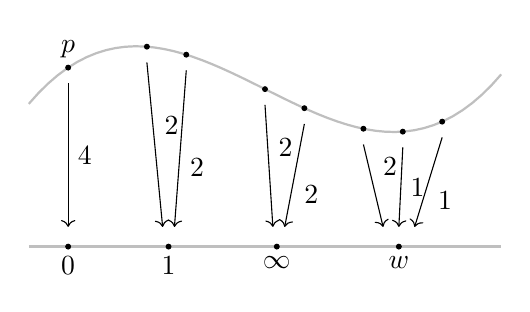
\begin{tikzpicture}[scale=0.50]
  \draw[domain=-6:6,samples=50,color=gray!50,thick] plot (\x, \x^3/64 - \x/2);
  \foreach \x/\p/\l in {-5/$p$/4}
  {
    \filldraw[black] (\x,\x^3/64 - \x/2) circle (0.6mm) node[above] {\p};
    \draw[->] (\x,\x^3/64 - \x/2 - .4) to["$\l$"] (-5, -3.5);
  }
  \foreach \x/\p/\l in {-3//2, -2//2}
  {
    \filldraw[black] (\x,\x^3/64 - \x/2) circle (0.6mm) node[above] {\p};
    \draw[->] (\x,\x^3/64 - \x/2 - .4) to["$\l$"] (-1.7+.3*\x, -3.5);
  }
  \foreach \x/\p/\l in {0//2, 1//2}
  {
    \filldraw[black] (\x,\x^3/64 - \x/2) circle (0.6mm) node[above] {\p};
    \draw[->] (\x,\x^3/64 - \x/2 - .4) to["$\l$"] (.2+.3*\x, -3.5);
    }
  \foreach \x/\p/\l in {2.5//2, 3.5//1, 4.5//1}
  {
    \filldraw[black] (\x,\x^3/64 - \x/2) circle (0.6mm) node[above] {\p};
    \draw[->] (\x,\x^3/64 - \x/2 - .4) to["$\l$"] (2+.4*\x, -3.5);
    }

    \draw[domain=-6:6,samples=50,color=gray!50,thick] plot (\x, -4);
  \foreach \x/\q in {-5/$0$, -2.45/$1$, .3/$\infty$, 3.4/$w$}
    \filldraw[black] (\x,-4) circle (0.6mm) node[below] {\q};
\end{tikzpicture}

\end{figure}
                                                                                                                                                                                                                          \end{frame}

                                                                                                                                                                                                                          \begin{frame}{Comparing different counts}

                                                                                                                                                                                                                            \begin{itemize}
                                                                                                                                                                                                                            \item Cela, Pandharipande, and Schmitt: Hurwitz numbers and Tevelev degrees provide information about the pushforward
                                                                                                                                                                                                                              of the fundamental class of the Hurwitz moduli space:
                                                                                                                                                                                                                                \[\begin{tikzcd}[ampersand replacement=\&]
	{\overline{\mathcal H}_{1,\sigma}} \& {\overline{\mathcal M}_{1,N}} \\
	{\overline{\mathcal M}_{0,n}} \& {\overline{\mathcal M}_{1,m}}
	\arrow["{\epsilon_1}", from=1-1, to=1-2]
	\arrow["{\epsilon_0}"', from=1-1, to=2-1]
	\arrow["{\pi_{\nu}}"', from=1-1, to=2-2]
	\arrow["\iota", from=1-2, to=2-2]
                                                                                                                                                                                                                                \end{tikzcd}\]
Product map $\tau=(\epsilon_0,\epsilon_g):\overline{\mathcal H}_{1,\sigma}\to\overline{\mathcal M}_{1,N}\times\overline{\mathcal M}_{0,n}$

                                                                                                                                                                                                                              \item Hurwitz number: fixed {\color{red}target} ($H=\deg(\epsilon_0)$)
                                                                                                                                                                                                                              \item Generalized Tevelev degree: partially fixed {\color{red}target}, partially fixed {\color{green!70!black}source}
                                                                                                                                                                                                                                \item My invariants $N_{1,\sigma,\nu}$: (partially) fixed {\color{green!70!black}source}
  
                                                                                                                                                                                                                            \end{itemize}
                                                                                                                                                                                                                            All give partial information about the pushforward $\tau_*[\overline{\mathcal H}_{1,\sigma}]$
                                                                                                                                                                                                                          \end{frame}

%                                                                                                                                                                                                                          \begin{frame}{Main results}

%                                                                                                                                                                                                                            \begin{itemize}
%                                                                                                                                                                                                                                \item Given
%  an even degree $d=2k$, a partition $\mu=(\mu_1,\dots,\mu_r)$ of $d$, and a generic
%  $r$-pointed genus $1$ curve $(C,p_1,\dots,p_r)$, we ask how many maps
%  $f:C\to\P^1$ exist with $f^{-1}(0)=\{p_1,\dots,p_r\}$, ramification index $\mu_i$
%  at $p_i$, and ramification profiles $(2,\dots,2)$ over both $1$ and $\infty\in\P^1$.
%  We show the answer to this ``even ramification'' problem is $3\cdot 2^{r-1}$.
%  \item Given
%  a degree $d$, a partition $\mu=(\mu_1,\dots,\mu_k)$ of $d$, multisets of positive integers $\a=\{a_1,\dots,a_r\}$ and $\b=\{b_1,\dots,b_s\}$,
%  and a generic $(k+s)$-pointed genus $1$ curve $(C,p_1,\dots,p_k,P_1,\dots,P_s)$,
%  we ask how many maps $f:C\to\P^1$ exist with $f^{-1}(0)=\{p_1,\dots,p_k\}$, ramification
%  index $\mu_i$ at $p_i$, ramification index $b_i$ at $P_i$, and other (unmarked) points
%  with ramification indices $a_1,\dots,a_r$. We establish recursive relations to compute these invariants.
%  \begin{itemize}
%    \item When $d=k+2$, $\a=\{3,\dots,3\}$ ($k$ copies), $\b=\emptyset$, we have a closed form
%    \end{itemize}
  
                                                                                                                                                                                              %                              \end{itemize}
                                                                                                                                                                                             %                             \end{frame}

                                                                                                                                                                                                                          \begin{frame}{Methods}
                                                                                                                                                                                                                            To compute $N_{1,\sigma,\nu}$:
                                                                                                                                                                                                                            \begin{itemize}
                                                                                                                                                                                                                            \item {\bf Direct evaluation:} if $\nu_1=\sigma_1$, maps $E\to\P^1$ can be written $E\hookrightarrow\P^d\dashrightarrow \ell=\P^1$
                                                                                                                                                                                                                              with line bundle $\mathcal L=\mathcal O(\sigma_1)$,
                                                                                                                                                                                                                              and we count lines $\ell\subset\P^d$ satisfying some conditions
                                                                                                                                                                                                                            \item {\bf Factoring:} if we're lucky, we can factor our maps as $E\to\P^1\to\P^1$ and perform simpler counts
                                                                                                                                                                                                                            \item {\bf Admissible covers:} we apply the method of (CITE), counting the number of admissible covers from a non-generic
                                                                                                                                                                                                                              {\it stable} curve
                                                                                                                                                                                                                            \end{itemize}
                                                                                                                                                                                                                          \end{frame}

                                                                                                                                                                                                                          \begin{frame}{Methods (example)}
      \begin{columns}[c]
        \begin{column}{0.3\hsize}
                                                                                                                                                                                                                            \begin{itemize}
                                                                                                                                                                                                                            \item {\bf Direct evaluation:} embed $E\hookrightarrow\P^3$, count lines $\ell\subset\P^3$
                                                                                                                                                                                                                              such that $p\notin\ell\subset H_0$, $\ell\subset H_1$, $\ell\subset H_2$ where $H_0\cap E=4p$, $H_1\cap E=2q+2r$, $H_2\cap E=2s+2t$
                                                                                                                                                                                                                            \item {\bf Factoring:} second map determined by choice
                                                                                                                                                                                                                              of $q_2$ and $q_3$: $\binom 32=3$
                                                                                                                                                                                                                            \end{itemize}
        \end{column}
        \begin{column}{0.7\hsize}

                                                                                                                                                                                                                                      \begin{figure}[h]
  \centering
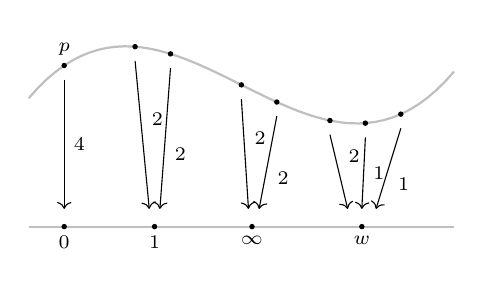
\begin{tikzpicture}[scale=0.45, font=\scriptsize]
  \draw[domain=-6:6,samples=50,color=gray!50,thick] plot (\x, \x^3/64 - \x/2);
  \foreach \x/\p/\l in {-5/$p$/4}
  {
    \filldraw[black] (\x,\x^3/64 - \x/2) circle (0.6mm) node[above] {\p};
    \draw[->] (\x,\x^3/64 - \x/2 - .4) to["$\l$"] (-5, -3.5);
  }
  \foreach \x/\p/\l in {-3//2, -2//2}
  {
    \filldraw[black] (\x,\x^3/64 - \x/2) circle (0.6mm) node[above] {\p};
    \draw[->] (\x,\x^3/64 - \x/2 - .4) to["$\l$"] (-1.7+.3*\x, -3.5);
  }
  \foreach \x/\p/\l in {0//2, 1//2}
  {
    \filldraw[black] (\x,\x^3/64 - \x/2) circle (0.6mm) node[above] {\p};
    \draw[->] (\x,\x^3/64 - \x/2 - .4) to["$\l$"] (.2+.3*\x, -3.5);
    }
  \foreach \x/\p/\l in {2.5//2, 3.5//1, 4.5//1}
  {
    \filldraw[black] (\x,\x^3/64 - \x/2) circle (0.6mm) node[above] {\p};
    \draw[->] (\x,\x^3/64 - \x/2 - .4) to["$\l$"] (2+.4*\x, -3.5);
    }

    \draw[domain=-6:6,samples=50,color=gray!50,thick] plot (\x, -4);
  \foreach \x/\q in {-5/$0$, -2.45/$1$, .3/$\infty$, 3.4/$w$}
    \filldraw[black] (\x,-4) circle (0.6mm) node[below] {\q};
\end{tikzpicture}

\label{fig:firsteg}
\end{figure}

                                                                                                                                                                                                                          \begin{figure}[h]
  \centering
  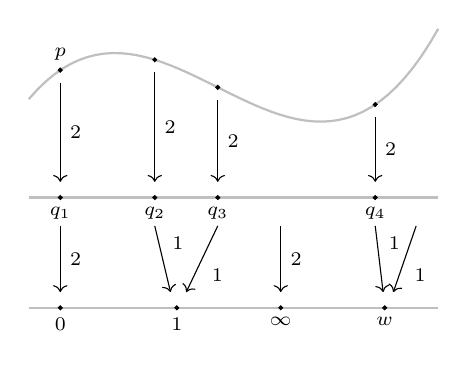
\begin{tikzpicture}[scale=0.4, font=\scriptsize]
  \draw[domain=-6:7.0,samples=50,color=gray!50,thick] plot (\x, \x^3/64 - \x/2); % Curve E
  \draw[domain=-6:7.0,samples=50,color=gray!50,thick] plot (\x, -3.5); % first P^1
  \draw[domain=-6:7.0,samples=50,color=gray!50,thick] plot (\x, -7); % second P^1

  % top map arrows and labels
  \foreach \p/\plabel/\qlabel in {-5/$p$/$q_1$, -2//$q_2$, 0//$q_3$, 5//$q_4$} {
    \filldraw[black] (\p, \p^3/64-\p/2) circle (0.6mm) node[above] {\plabel};
    \draw[->] (\p, \p^3/64-\p/2-.4) to["2"] (\p, -3);
    \filldraw[black] (\p, -3.5) circle (0.6mm) node[below] {\qlabel};
  }

  % fiber over 0
  \draw[->] (-5, -4.4) to["$2$"] (-5, -6.5);

  % fiber over 1
  \foreach \x/\l in {-2/$1$, 0/$1$} {
    \draw[->] (\x, -4.4) to["\l"] (-1+\x/4, -6.5);
  }

    % fiber over infinity
  \foreach \x/\l in {2/$2$} {
    \draw[->] (\x, -4.4) to["\l"] (3/2+\x/4, -6.5);
  }

  % fiber over w
  \foreach \x/\l in {5/$1$, 6.3/$1$} {
    \draw[->] (\x, -4.4) to["\l"] (4+\x/4, -6.5);
  }

  % 0, 1, infinity, w
  \foreach \x/\l in {-5/$0$, -1.3/$1$, 2/$\infty$, 5.3/$w$} {
    \filldraw[black] (\x, -7) circle (0.6mm) node[below] {\l};
    }

\end{tikzpicture}

\label{fig:comb2}
                                                                                                                                                                                                                          \end{figure}
        \end{column}
        \end{columns}
                                                                                                                                                                                                                          \end{frame}

                                                                                                                                                                                                                          \begin{frame}{Admissible covers}
                                                                                                                                                                                                                            Replace elliptic curve with a pointed genus $1$ nodal curve:
                                                                                                                                                                                                                            \includegraphics[scale=0.16]{nodal.png}


                                                                                                                                                                                                                            $N_{1,\sigma,\nu}={\color{brown}1}+{\color{magenta}2}=3$
      \begin{columns}[c]
        \begin{column}{0.5\hsize}
          \begin{figure}
          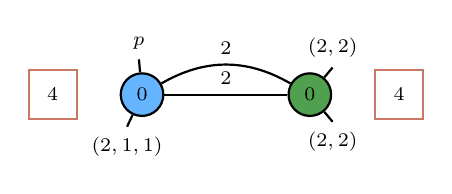
\begin{tikzpicture}[font=\scriptsize,thick,amat/.style={matrix of nodes,nodes in empty cells,
  row sep=.5em,rounded corners,
  nodes={draw,solid,circle,minimum size=0.3cm}},
  dmat/.style={matrix of nodes,nodes in empty cells,row sep=.5em,nodes={minimum size=0.3cm},draw=myred},
  fsnode/.style={fill=myblue},
  ssnode/.style={fill=mygreen}]

  \matrix[amat,nodes=fsnode] (mat1) {$0$\\};

    \matrix[dmat,left=0.4cm of mat1] (degrees1) {$4$\\};


 \matrix[amat,right=1.3cm of mat1,nodes=ssnode] (mat2) {$0$\\};

 \matrix[dmat,right=0.4cm of mat2] (degrees2) {$4$\\};

 \draw  (mat1-1-1) edge["$2$",bend left] (mat2-1-1)
 (mat1-1-1) edge["$2$"] (mat2-1-1);

  % draw legs for left side
 \draw (mat1-1-1) -- +(95:.45) node[anchor=south] {$p$}
 (mat1-1-1) -- +(245:.45) node[anchor=north] {$(2,1,1)$};

 % draw legs for right side
 \draw  (mat2-1-1) -- +(50:.45) node[anchor=south] {$(2,2)$}
 (mat2-1-1) -- +(310:.45) node[anchor=north] {$(2,2)$};

          \end{tikzpicture}
          \end{figure}
\begin{center}{\color{brown}\Large $1$}\end{center}
          
        \end{column}
        \begin{column}{0.5\hsize}
            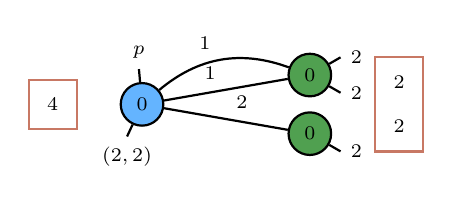
\begin{tikzpicture}[font=\scriptsize,thick,amat/.style={matrix of nodes,nodes in empty cells,
  row sep=.5em,rounded corners,
  nodes={draw,solid,circle,minimum size=0.3cm}},
  dmat/.style={matrix of nodes,nodes in empty cells,row sep=.5em,nodes={minimum size=0.3cm},draw=myred},
  fsnode/.style={fill=myblue},
  ssnode/.style={fill=mygreen}]

  \matrix[amat,nodes=fsnode] (mat1) {$0$\\};

    \matrix[dmat,left=0.4cm of mat1] (degrees1) {$4$\\};


 \matrix[amat,right=1.3cm of mat1,nodes=ssnode] (mat2) {$0$\\
      $0$\\};

 \matrix[dmat,right=0.4cm of mat2] (degrees2) {$2$\\
   $2$ \\};

 \draw  (mat1-1-1) edge["$1$",bend left] (mat2-1-1)
 (mat1-1-1) edge["$1$"] (mat2-1-1)
 (mat1-1-1) edge["$2$"] (mat2-2-1);

  % draw legs for left side
 \draw (mat1-1-1) -- +(95:.45) node[anchor=south] {$p$}
 (mat1-1-1) -- +(245:.45) node[anchor=north] {$(2,2)$};

 % draw legs for right side
 \draw  (mat2-1-1) -- +(30:.45) node[anchor=west] {$2$}
 (mat2-1-1) -- +(330:.45) node[anchor=west] {$2$}
 (mat2-2-1) -- +(330:.45) node[anchor=west] {$2$};

            \end{tikzpicture}

            \begin{center}{\color{magenta}\Large $2$}\end{center}
        \end{column}
        \end{columns}
                                                                                                                                                                                                                          \end{frame}

                                                                                                                                                                                                                          \begin{frame}{Some values}

                                                                                                                                                                                                                            Letting $N_{\sigma_1,\dots,\sigma_n}(\mu)$ be an invariant with ramification
                                                                                                                                                                                                                            profiles $\sigma_1,\dots,\sigma_n,\mu$ and where the points corresponding to $\mu$ are fixed:
                                                                                                                                                                                                                            \begin{table}[h]
    \caption{Table of invariants for $n=4$.}
    \centering
    ~\\
\begin{tabular}{|l|l|l|l|l|}
\hline
$\mu$             & $N_{(4)}(\mu)$ & $N_{(3,1),(2,2)}(\mu)$ & $N_{(2,2),(2,2)}(\mu)$ & $N_{(3,1),(3,1)}(\mu)$ \\ \hline
{4} & {15} & {18}        & {3}         & {20}        \\ \hline
3,1                     & {16} & {32}        & {6}         & {28}        \\ \hline
2,2                     & {16} & {18}        & {6}         & {36}        \\ \hline
2,1,1                   & {16} & {36}        & {12}        & {37}        \\ \hline
1,1,1,1                 & {16} & {48}        & {24}        & {38}        \\ \hline
\end{tabular}
\end{table}
                                                                                                                                                                                                                            \end{frame}
                                                                                                                                                                                                                          \begin{frame}{All twos case}
                                                                                                                                                                                                                            \begin{itemize}
                                                                                                                                                                                                                              \item
                                        Given
  an even degree $d=2k$, a partition $\mu=(\mu_1,\dots,\mu_r)$ of $d$, and a generic
  $r$-pointed genus $1$ curve $(E,p_1,\dots,p_r)$, let $N_{(2^k),(2^k)}(\mu)$ be the number of covers
  $f:E\to\P^1$ with $f^{-1}(0)=\{p_1,\dots,p_r\}$, ramification index $\mu_i$
  at $p_i$, and ramification profiles $(2,\dots,2)$ over both $1$ and $\infty\in\P^1$. Then $N_{(2^k),(2^k)}(\mu)={\boxed{3\cdot 2^{r-1}}}$.
\item Proof idea: if $r\geq 2$, count admissible covers from a stable curve with a rational tail containing $p_1,p_2$;
  yields a recursion
                                                                                                                                                                                                                            \end{itemize}
  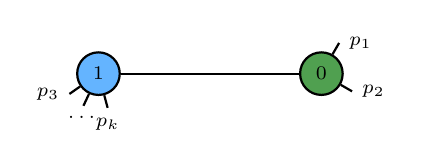
\begin{tikzpicture}[font=\scriptsize,thick,amat/.style={matrix of nodes,nodes in empty cells,
  row sep=2.5em,rounded corners,
  nodes={draw,solid,circle,minimum size=0.5cm}},
  dmat/.style={matrix of nodes,nodes in empty cells,row sep=2.5em,nodes={minimum size=0.5cm},draw=myred},
  fsnode/.style={fill=myblue},
  ssnode/.style={fill=mygreen}]

  \matrix[amat,nodes=fsnode] (mat1) {$1$\\};

 \matrix[amat,right=2cm of mat1,nodes=ssnode] (mat2) {$0$\\};

 \draw  (mat1-1-1) edge (mat2-1-1);

  % draw legs for left side
 \draw (mat1-1-1) -- +(215:.45) node[anchor=east] {$p_{3}$}
 (mat1-1-1) -- +(245:.45) node[anchor=north] {$\dots$}
 (mat1-1-1) -- +(285:.45) node[anchor=north] {$p_{k}$};

 % draw legs for right side
 \draw  (mat2-1-1) -- +(60:.45) node[anchor=west] {$p_{1}$}
 (mat2-1-1) -- +(330:.45) node[anchor=west] {$p_{2}$};

  \end{tikzpicture}

  E.g. $N_{(2,2,2),(2,2,2)}(4,1,1)=N_{(2,2,2),(2,2,2)}(5,1)+N_{(2,2),(2,2)}(3,1)$
                                                                                                                                                                                                                          \end{frame}

                                                                                                                                                                                                                          \begin{frame}{$S_{\a,\b}$}

                                                                                                                                                                                                                            Given
  a degree $d$, a partition $\mu=(\mu_1,\dots,\mu_k)$ of $d$, multisets of positive integers $\a=\{a_1,\dots,a_r\}$ and $\b=\{b_1,\dots,b_s\}$,
  and a generic $(k+s)$-pointed genus $1$ curve $(E,p_1,\dots,p_k,P_1,\dots,P_s)$,
  $S_{\a,\b}$ is the number of covers $f:E\to\P^1$ with $f^{-1}(0)=\{p_1,\dots,p_k\}$, ramification
  index $\mu_i$ at $p_i$, ramification index $b_i$ at $P_i$, and other (unmarked) points
  with ramification indices $a_1,\dots,a_r$:

    \begin{figure}[h]
  \centering
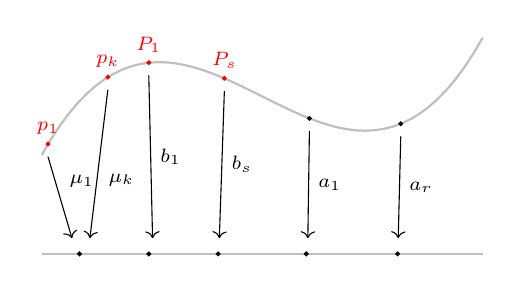
\begin{tikzpicture}[scale=0.4,font=\scriptsize]
  \draw[domain=-7:7,samples=50,color=gray!50,thick] plot (\x, \x^3/64 - \x/2);
  \foreach \x/\p/\c/\d in {-6.8/$p_1$/red/$\mu_1$, -4.9/$p_k$/red/$\mu_k$}
  {
    \filldraw[\c] (\x,\x^3/64 - \x/2) circle (0.6mm) node[above] {\p};
    \draw[->] (\x,\x^3/64 - \x/2 - .4) to["\d"] (-4+.3*\x, -4.5);
  }

  \foreach \x/\p/\c/\d in {-3.6/$P_1$/red/$b_1$}
  {
    \filldraw[\c] (\x,\x^3/64 - \x/2) circle (0.6mm) node[above] {\p};
    \draw[->] (\x,\x^3/64 - \x/2 - .4) to["\d"] (-2.4+.3*\x, -4.5);
  }
  
  \foreach \x/\p/\c/\d in {-1.2/$P_{s}$/red/$b_s$}
  {
    \filldraw[\c] (\x,\x^3/64 - \x/2) circle (0.6mm) node[above] {\p};
    \draw[->] (\x,\x^3/64 - \x/2 - .4) to["\d"] (-1+.3*\x, -4.5);
  }

  \foreach \x/\p/\c/\d in {1.5//black/$a_1$}
  {
    \filldraw[\c] (\x,\x^3/64 - \x/2) circle (0.6mm) node[above] {\p};
    \draw[->] (\x,\x^3/64 - \x/2 - .4) to["\d"] (1+.3*\x, -4.5);
  }
  
  \foreach \x/\p/\c/\d in {4.4//black/$a_r$}
  {
    \filldraw[\c] (\x,\x^3/64 - \x/2) circle (0.6mm) node[above] {\p};
    \draw[->] (\x,\x^3/64 - \x/2 - .4) to["\d"] (3+.3*\x, -4.5);
    }

    \draw[domain=-7:7,samples=50,color=gray!50,thick] plot (\x, -5);
  \foreach \x/\q in {-5.8/$q_1$, -3.6/$q_2$, -1.4/$q_3$, 1.4/$q_4$, 4.3/$q_5$}
    \filldraw[black] (\x,-5) circle (0.6mm) node[below]{};
\end{tikzpicture}

(Red points fixed)

\label{fig:Sab}
  \end{figure}
                                                                                                                                                                                                                          \end{frame}

                                                                                                                                                                                                                          \begin{frame}{$S_{\a,\b}$ (continued)}

                                                                                                                                                                                                                            Results:
                                                                                                                                                                                                                            \begin{itemize}
                                                                                                                                                                                                                            \item  Recursive formulas reducing $\a$ and $\b$, e.g.
                                 \tiny{                                                                                                                                                                                             \[
                                   S_{\mathfrak a,\mathfrak b+\{y\}}(\mu, n) =S_{\mathfrak a,\mathfrak b}(\mu, n-y+1) +\sum_{z\in\mathfrak a}\min(z-1,y-1,n,y+z-n-2)S_{\mathfrak a-\{z\},\mathfrak b+\{y+z-n-2\}}(\mu)                                                                                                                                                                                           \]}
                                 \normalsize\item {Along with base case $\b=\emptyset$ and $\ell(\a)=1$, these allow us to compute any $S_{\a,\b}$}
                               \item Special case:
                                 \[
                                 S_{\{3\}^k,\emptyset}(1^{k+2})=\frac{(k+2)(k+1)(2(k+1)^2+1)}{6}
                                 \]
                                                                                                                                                                                                                            \end{itemize}
                                                                                                                                                                                                                          \end{frame}
                                                                                                                                                                                                                          \begin{frame}{Conclusions}
                                                                                                                                                                                                                            \begin{itemize}
                                                                                                                                                                                                                            \item We have effective methods to compute $N_{1,\sigma,\nu}$ in special families. The general problem seems hard.
                                                                                                                                                                                                                            \item Possible future directions:
                                                                                                                                                                                                                              \begin{itemize}

                                                                                                                                                                                                                              \item Better understanding $S_{\{n\}^k,\emptyset}(1^{k(n-2)+2})$ and its asymptotics (known quartic for $n=3$, likely
                                                                                                                                                                                                                                exponential growth in $k$ for $n>3$)
                                                                                                                                                                                                                              \item Similar invariants with $g\neq 1$
                                                                                                                                                                                                                              \item Cohomology classes: $N_{(2^k),(2^k)}(\mu)$ is only one relative Gromov-Witten invariant of the pillowcase orbifold $C=\P^1/\Z_2$,
                                                                                                                                                                                                                                and there is a larger family $\langle \mu\rangle_d^{C}\in H^{g-1}(\overline{\mathcal M}_{g,\ell(\mu)})$
                                                                                                                                                                                                                              \end{itemize}
                                                                                                                                                                                                                            \end{itemize}
                                                                                                                                                                                                                          \end{frame}

                                                                                                                                                                                                                          \begin{frame}{References}
                                          x                                                                                                                                                                                  \end{frame}

\end{document}
